%!TEX root = ./template-skripsi.tex
\subsection{\textit{Sprint 3}}

	\textit{Sprint-3} dilakukan sepekan pada tanggal 6 September 2022 sampai dengan 13 September 2022. \textit{Story} ketiga  pada \textit{product backlog} yaitu membuat fitur pemberian pakan, ditambah dengan melanjutkan bagian yang belum selesai dari sprint sebelumnya yaitu mengintegrasikan halaman list kolam, registrasi kolam, aktivasi kolam, dan deaktivasi kolam dipecah menjadi beberapa \textit{task} sebagai berikut.


 \begin{longtable}[c]{@{} |p{1cm}|p{4cm}|p{5cm}|p{3cm}| @{}}
 \caption{\textit{Sprint 3} \label{sprint3_table}}\\


 \hline
  \multirow{1}{=}{\centering{\textbf{No}}} & \multirow{1}{=}{\centering{\textbf{\textit{Story}}}} & \multirow{1}{=}{\centering{\textbf{\textit{Task}}}} & \multirow{1}{=}{\centering{\textbf{\textit{Status}}}}\\
 \endfirsthead

 \hline
  \multirow{1}{=}{\centering{\textbf{No}}} & \multirow{1}{=}{\centering{\textbf{\textit{Story}}}} & \multirow{1}{=}{\centering{\textbf{\textit{Task}}}} & \multirow{1}{=}{\centering{\textbf{\textit{Status}}}}\\
 \endhead

 \hline
 \endfoot

 \hline
 \endlastfoot

 \hline
 1 & Melanjutkan bagian yang belum selesai dari sprint sebelumnya &  Mengintegrasikan halaman list kolam, registrasi kolam, aktivasi kolam, dan deaktivasi kolamm &  selesai \\
 \hline
 2 & Membuat fitur pemberian pakan & Membuat mockup-UI untuk fitur pemberian pakan & selesai\\
 \hline
 3 & & Menerapkan \textit{Mock-up UI} halaman pemberian pakan & selesai\\
 \hline
 4 & & Mengintegrasikan halaman pemberian pakan ke \textit{webservice} & selesai\\
 \hline
 \end{longtable}

Pada \textit{sprint-3} ini, story yang dipilih untuk diuraikan adalah membuat fitur pemberian pakan pada kolam budidaya. Tujuan dari \textit{sprint-3} adalah membuat fitur pemberian pakan, serta mengintegrasikan halaman-halaman tersebut dengan webservice. Kendala yang dialami penulis pada \textit{sprint-3} ini adalah banyaknya fitur yang harus diaplikasikan sehingga ada beberapa task yang harus dilanjutkan pada \textit{sprint} berikutnya. Berikut merupakan hasil dari pengerjaan yang dilakukan selama \textit{sprint 3}.

\begin{enumerate}[listparindent=2em]

	\item {\textit{Mengintegrasikan halaman list kolam, registrasi kolam, aktivasi kolam, deaktivasi kolam dengan webservice}}

  sebelumnya data yang terdapat pada halaman list kolam, registrasi kolam, aktivasi kolam, deaktivasi kolam masih berupa data dummy, maka dari itu pada sprint ini penulis perlu mengintegrasikan halaman tersebut dengan web service, code tersebut dapat dilihat pada lampiran 4.


	\item{\textit{Membuat Mock-up UI Halaman Pemberian pakan}}
	
	Pembuatan konten dan fitur yang terdapat pada \textit{mock-up UI} halamanpemberian pakan dilakukan berdasarkan persetujuan product owner dan scrum master pada meeting sebelumnya. Mock-up UI dibuat menggunakan platform figma.
	
	\begin{figure}[H]
	\centering
	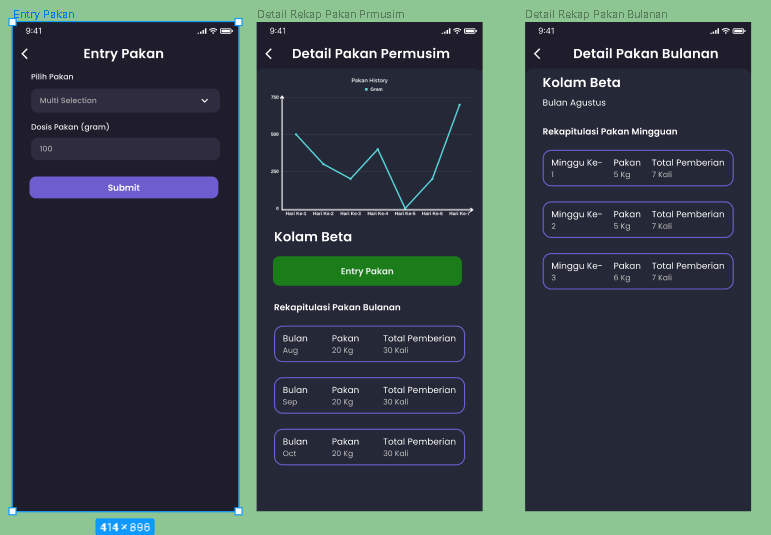
\includegraphics[keepaspectratio, width=4cm]{gambar/ssmockuppakan}
	\caption{\textit{Mock-up UI pemberian pakan}}
	\label{gambar:mockupsprint3}
	\end{figure}

	\item{\textit{Menerapkan mockup-UI  halaman pemberian pakan, rekapitulasi pakan kedalam code flutter}}
	
	Setelah \textit{mock-up UI  pemberian pakan, rekapitulasi pakan} dibuat, akan dilakukan pengimplementasian \textit{mock- up UI} ke dalam aplikasi menggukan flutter. Berikut adalah source code dari implementasi halaman  pemberian pakan, rekapitulasi pakan yang dikelompokan pada lampiran 4 dan menghasilkan output sebagai berikut.

	\begin{figure}[H]
	\centering
	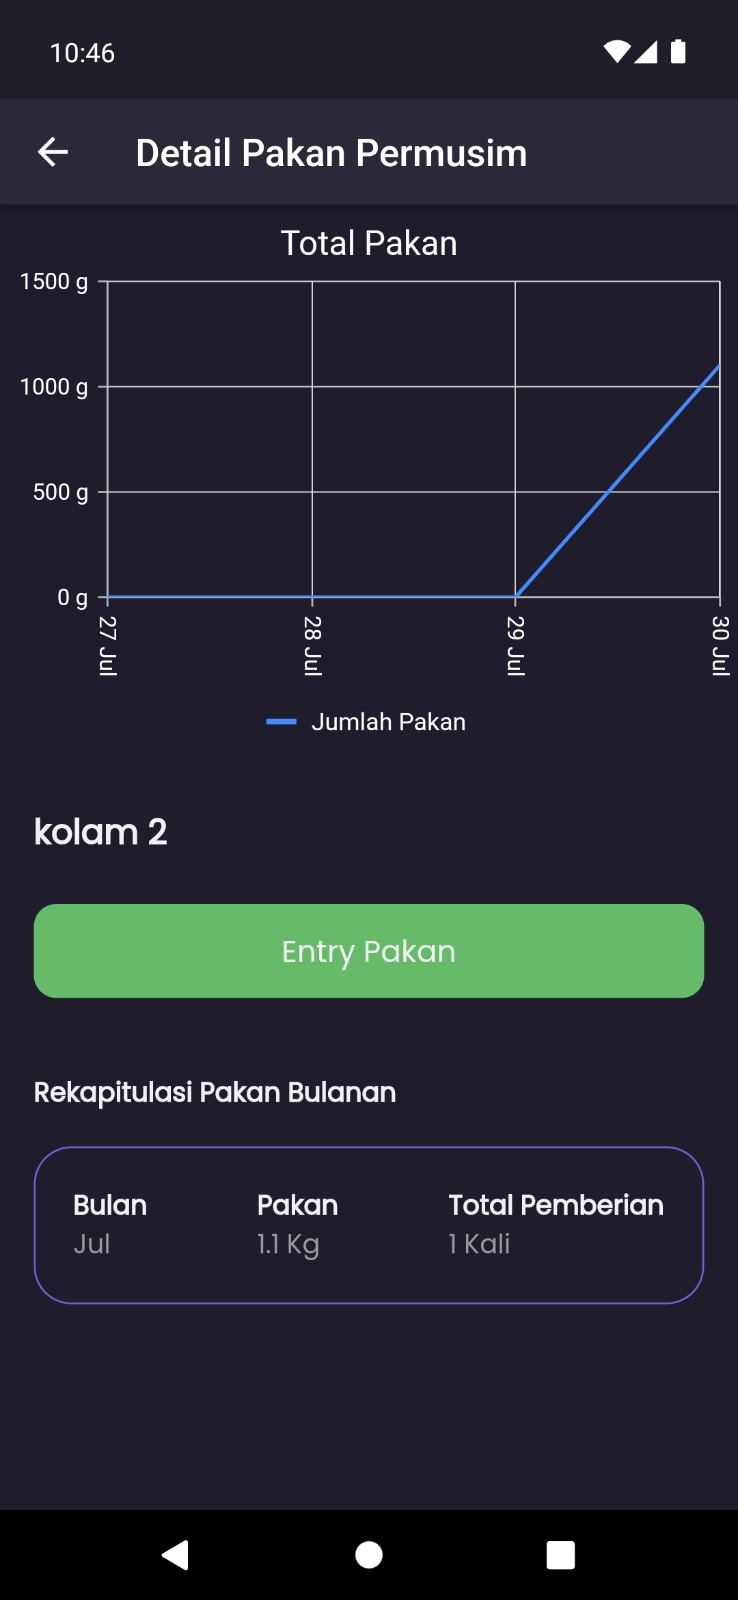
\includegraphics[keepaspectratio, width=3cm]{gambar/ssrekappakan}
	\caption{\textit{Output dari code pada rekapitulasi pakan}}
	\label{gambar:ssrekappakan}
	\end{figure}
	
	\begin{figure}[H]
	\centering
	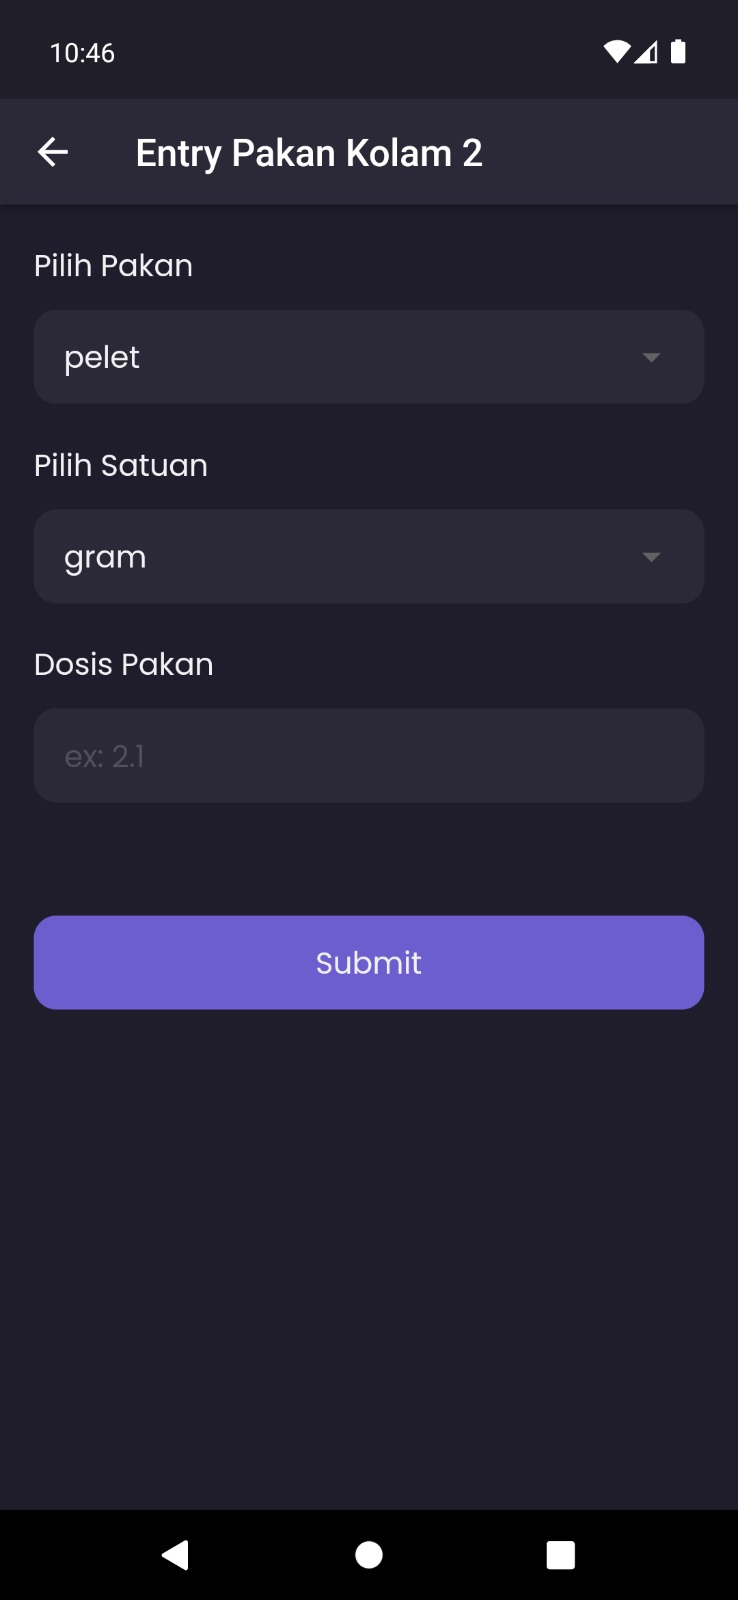
\includegraphics[keepaspectratio, width=4cm]{gambar/ssentrypakan}
	\caption{\textit{Output dari code untuk halaman entry pakan}}
	\label{gambar:ssentrypakan}
	\end{figure}

	\item{\textit{Mengitegrasikan fitur pemberian pakan dengan webservice}}

	Sebelumnya, setiap data pada fitur masih berupa data dummy sehingga perlu diintegrasikan dengan webservice agar aplikasi dapat berjalan dengan data yang asli. Hal yang dilakukan dalam mengintegrasikan fitur pemberian pakan dengan webservice terdapat pada lampiran 4.

  \item{Analisis \textit{User Experience}} 
 
Pada halaman pemberian pakan, pembudidaya harus memasukan dosis pakan dan jenis pakan yang diberikan sehingga data tersbut dapat diolah untuk output FCR nanti saat panen. Di halaman rekapitulasi pakan, terdapat grafik mengenai statistik jumlah pakan yang telah diberikan pada musim budidaya yang berjalan sehingga pembudidaya dapat dengan mudah mengetahui statistik rekap pakan dari setiap musim budidaya yang berjalan, selain itu terdapat juga list mengenai pakan yang telah diberikan yang berisi informasi dosis dan waktu pembudidaya saat memberikan pakan.


\item{Sprint 3 Review dan Sprint 4 Planning}

Sprint 3 diakhiri dengan melakukan weekly meeting pada hari selasa dengan agenda melakukan review dan testing terkait hasil sprint 3 dan melakukan planning untuk sprint 4 dengan rincian:
\begin{enumerate}
	\item{\textit{Review dan Testing hasil dari sprint 3}}

  Telah dilakukan review dan testing oleh penulis selaku developer dengan Scrum Master. Setelah dilakukan testing, Scrum Master menyimpulkan bahwa penerapan fitur pemberian pakan telah berjalan dengan baik.
  
\begin{longtable}{| p{8cm} | c | c | l |}
  \caption{Unit testing Halaman Daftar Kolam.\label{table:unit_testing_fitur_daftar_kolam}}\\
  \hline
  \multirow{2}{*}{Skenario Pengujian} & \multicolumn{2}{l|}{Kesesuaian} & \multirow{2}{*}{Kesimpulan} \\ 
  \cline{2-3}
    & \multicolumn{1}{l|}{sesuai} & tidak sesuai & \\ 
  \hline
  \hline
  \endfirsthead
  \hline
  \multirow{2}{*}{Skenario Pengujian} & \multicolumn{2}{l|}{Kesesuaian} & \multirow{2}{*}{Kesimpulan} \\ 
  \cline{2-3}
    & \multicolumn{1}{l|}{sesuai} & tidak sesuai &  \\ 
  \hline
  \hline
  \endhead
  \hline
  \endfoot
  
  
  \hline\hline
  \endlastfoot
   Saat ikon (+) ditekan maka akan menampilkan halaman registrasi kolam & \Checkmark &  & Diterima \\ 
  \hline
   Saat card kolam ditekan akan menampilkan halaman detail kolam & \Checkmark & & Diterima \\ 
  \hline
  \end{longtable}
  
  \begin{longtable}{| p{8cm} | c | c | l |}
  \caption{Unit testing Halaman Registrasi Kolam.\label{table:unit_testing_fitur_regis_kolam}}\\
  \hline
  \multirow{2}{*}{Skenario Pengujian} & \multicolumn{2}{l|}{Kesesuaian} & \multirow{2}{*}{Kesimpulan} \\ 
  \cline{2-3}
    & \multicolumn{1}{l|}{sesuai} & tidak sesuai & \\ 
  \hline
  \hline
  \endfirsthead
  \hline
  \multirow{2}{*}{Skenario Pengujian} & \multicolumn{2}{l|}{Kesesuaian} & \multirow{2}{*}{Kesimpulan} \\ 
  \cline{2-3}
    & \multicolumn{1}{l|}{sesuai} & tidak sesuai &  \\ 
  \hline
  \hline
  \endhead
  \hline
  \endfoot
  
  
  \hline\hline
  \endlastfoot
   ketika mengisi form registrasi kolam dengan data yang sesuai dan menekan submit, maka kolam baru akan ditambakan & \Checkmark &  & Diterima \\ 
  \hline
  \end{longtable}
  
  \begin{longtable}{| p{8cm} | c | c | l |}
  \caption{Unit testing Halaman Detail Kolam.\label{table:unit_testing_fitur_detail_kolam}}\\
  \hline
  \multirow{2}{*}{Skenario Pengujian} & \multicolumn{2}{l|}{Kesesuaian} & \multirow{2}{*}{Kesimpulan} \\ 
  \cline{2-3}
    & \multicolumn{1}{l|}{sesuai} & tidak sesuai & \\ 
  \hline
  \hline
  \endfirsthead
  \hline
  \multirow{2}{*}{Skenario Pengujian} & \multicolumn{2}{l|}{Kesesuaian} & \multirow{2}{*}{Kesimpulan} \\ 
  \cline{2-3}
    & \multicolumn{1}{l|}{sesuai} & tidak sesuai &  \\ 
  \hline
  \hline
  \endhead
  \hline
  \endfoot
  
  
  \hline\hline
  \endlastfoot
   ketika tombol kualitas air ditekan maka akan menampilkan halaman kualitas air & \Checkmark &  & Diterima \\ 
  \hline
   ketikan menekan salah satu list dari masa budidaya akan menampilkan halaman detail masa budidaya & \Checkmark &  & Diterima \\ 
  \hline
   ketika status kolam tidak aktif atau panen dan menekan tombol start budidaya, maka akan menampilkan halaman aktivasi kolam & \Checkmark &  & Diterima \\ 
  \hline
   ketika status kolam aktif dan menekan tombol aktif, maka akan menampilkan halaman deaktivasi kolam & \Checkmark &  & Diterima \\ 
  \hline
  \end{longtable}
  
  \begin{longtable}{| p{8cm} | c | c | l |}
  \caption{Unit testing Halaman Registrasi Kolam.\label{table:unit_testing_fitur_regis_kolam}}\\
  \hline
  \multirow{2}{*}{Skenario Pengujian} & \multicolumn{2}{l|}{Kesesuaian} & \multirow{2}{*}{Kesimpulan} \\ 
  \cline{2-3}
    & \multicolumn{1}{l|}{sesuai} & tidak sesuai & \\ 
  \hline
  \hline
  \endfirsthead
  \hline
  \multirow{2}{*}{Skenario Pengujian} & \multicolumn{2}{l|}{Kesesuaian} & \multirow{2}{*}{Kesimpulan} \\ 
  \cline{2-3}
    & \multicolumn{1}{l|}{sesuai} & tidak sesuai &  \\ 
  \hline
  \hline
  \endhead
  \hline
  \endfoot
  
  
  \hline\hline
  \endlastfoot
   ketika mengisi form registrasi kolam dengan data yang sesuai dan menekan submit, maka kolam baru akan ditambakan & \Checkmark &  & Diterima \\ 
  \hline
  \end{longtable}
  
  \begin{longtable}{| p{8cm} | c | c | l |}
  \caption{Unit testing Halaman Aktivasi Kolam.\label{table:unit_testing_fitur_aktivasi_kolam}}\\
  \hline
  \multirow{2}{*}{Skenario Pengujian} & \multicolumn{2}{l|}{Kesesuaian} & \multirow{2}{*}{Kesimpulan} \\ 
  \cline{2-3}
    & \multicolumn{1}{l|}{sesuai} & tidak sesuai & \\ 
  \hline
  \hline
  \endfirsthead
  \hline
  \multirow{2}{*}{Skenario Pengujian} & \multicolumn{2}{l|}{Kesesuaian} & \multirow{2}{*}{Kesimpulan} \\ 
  \cline{2-3}
    & \multicolumn{1}{l|}{sesuai} & tidak sesuai &  \\ 
  \hline
  \hline
  \endhead
  \hline
  \endfoot
  
  
  \hline\hline
  \endlastfoot
   ketika mengisi form aktivasi kolam dengan data yang sesuai dan menekan submit, maka musim budidaya baru akan ditambahkan dan status kolam menjadi aktif & \Checkmark &  & Diterima \\ 
  \hline
  \end{longtable}
  
  \begin{longtable}{| p{8cm} | c | c | l |}
  \caption{Unit testing Halaman Deaktivasi Kolam.\label{table:unit_testing_fitur_deaktivasi_kolam}}\\
  \hline
  \multirow{2}{*}{Skenario Pengujian} & \multicolumn{2}{l|}{Kesesuaian} & \multirow{2}{*}{Kesimpulan} \\ 
  \cline{2-3}
    & \multicolumn{1}{l|}{sesuai} & tidak sesuai & \\ 
  \hline
  \hline
  \endfirsthead
  \hline
  \multirow{2}{*}{Skenario Pengujian} & \multicolumn{2}{l|}{Kesesuaian} & \multirow{2}{*}{Kesimpulan} \\ 
  \cline{2-3}
    & \multicolumn{1}{l|}{sesuai} & tidak sesuai &  \\ 
  \hline
  \hline
  \endhead
  \hline
  \endfoot
  
  
  \hline\hline
  \endlastfoot
   ketika mengisi form deaktivasi kolam dengan data yang sesuai dan menekan submit, maka musim budidaya yang barjalan akan berhenti status kolam menjadi tidak aktif & \Checkmark &  & Diterima \\ 
  \hline
  \end{longtable}
  

  \begin{longtable}{| p{8cm} | c | c | l |}
    \caption{Unit testing Halaman Detail Masa Budidaya.\label{table:unit_testing_detail_budidaya}}\\
    \hline
    \multirow{2}{*}{Skenario Pengujian} & \multicolumn{2}{l|}{Kesesuaian} & \multirow{2}{*}{Kesimpulan} \\ 
    \cline{2-3}
      & \multicolumn{1}{l|}{sesuai} & tidak sesuai & \\ 
    \hline
    \hline
    \endfirsthead
    \hline
    \multirow{2}{*}{Skenario Pengujian} & \multicolumn{2}{l|}{Kesesuaian} & \multirow{2}{*}{Kesimpulan} \\ 
    \cline{2-3}
      & \multicolumn{1}{l|}{sesuai} & tidak sesuai &  \\ 
    \hline
    \hline
    \endhead
    \hline
    \endfoot
    
    
    \hline\hline
    \endlastfoot
    Ketika tombol rekapitulasi pakan ditekan, maka akan ditampilkan halaman rekapitulasi pakan & \Checkmark &  & Diterima \\ 
    \hline
    Ketika tombol rekapitulasi kematian ikan ditekan, maka akan ditampilkan halaman rekapitulasi kematian ikan & \Checkmark &  & Diterima \\ 
    \hline
    Ketika tombol rekapitulasi grading ikan ditekan, maka akan ditampilkan halaman rekapitulasi grading ikan & \Checkmark &  & Diterima \\ 
    \hline
    Ketika tombol treatment ditekan, maka akan ditampilkan halaman treatment kolam & \Checkmark &  & Diterima \\ 
    \hline
     Ketika tombol sortir ditekan, maka akan ditampilkan halaman sortir kolam & \Checkmark &  & Diterima \\ 
    \hline
    \end{longtable}
    
    
    \begin{longtable}{| p{8cm} | c | c | l |}
    \caption{Unit testing Halaman Rekapitulasi Pakan.\label{table:unit_testing_rekapitulasi_pakan}}\\
    \hline
    \multirow{2}{*}{Skenario Pengujian} & \multicolumn{2}{l|}{Kesesuaian} & \multirow{2}{*}{Kesimpulan} \\ 
    \cline{2-3}
      & \multicolumn{1}{l|}{sesuai} & tidak sesuai & \\ 
    \hline
    \hline
    \endfirsthead
    \hline
    \multirow{2}{*}{Skenario Pengujian} & \multicolumn{2}{l|}{Kesesuaian} & \multirow{2}{*}{Kesimpulan} \\ 
    \cline{2-3}
      & \multicolumn{1}{l|}{sesuai} & tidak sesuai &  \\ 
    \hline
    \hline
    \endhead
    \hline
    \endfoot
    
    
    \hline\hline
    \endlastfoot
    Ketika menekan list data rekapitulasi pakan, maka akan ditamplikan detail rekapitulasi pakan & \Checkmark &  & Diterima \\ 
    \hline
    Ketika menekan list data rekapitulasi pakan, maka akan ditamplikan detail rekapitulasi pakan & \Checkmark &  & Diterima \\ 
    \hline
    Saat tombol entry pakan ditekan maka akan menampilkan halaman entry pakan & \Checkmark &  & Diterima \\ 
    \hline
     ketika mengisi form rekapitulasi pakan dengan data yang sesuai dan menekan submit, data rekapitulasi pakan akan ditambahkan & \Checkmark &  & Diterima \\ 
    \hline
    \end{longtable}

	\item{\textit{Sprint Planning untuk Sprint 4}}
	
	Planning untuk sprint 4 yakni membuat fitur grading ikan pada aplikasi \textit{Assistive Aquaculture Breeding Management}.
\end{enumerate}
\end{enumerate}